\section{\uppercase{Proposed Method}} \label{sec3}
\begin{figure}[tb]
\centering
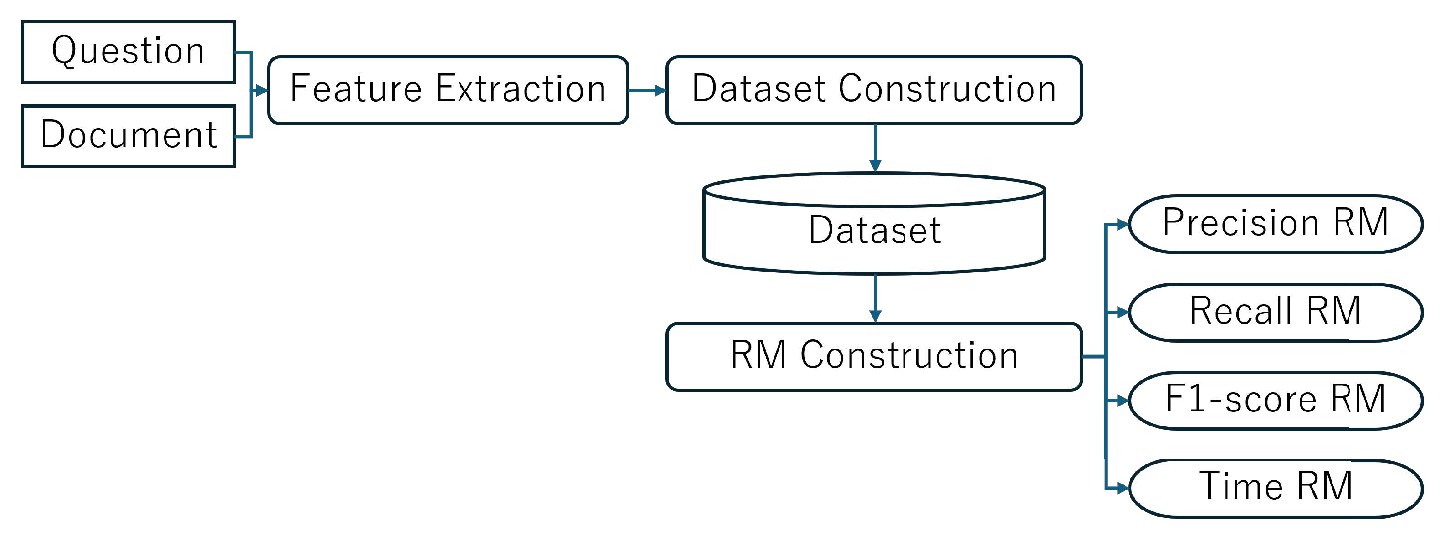
\includegraphics[width=\linewidth]{figures/Fig1}
\caption{Training procedure of ranking models in the proposed method.}
\label{construction}
\end{figure}

\begin{figure}[tb]
\centering
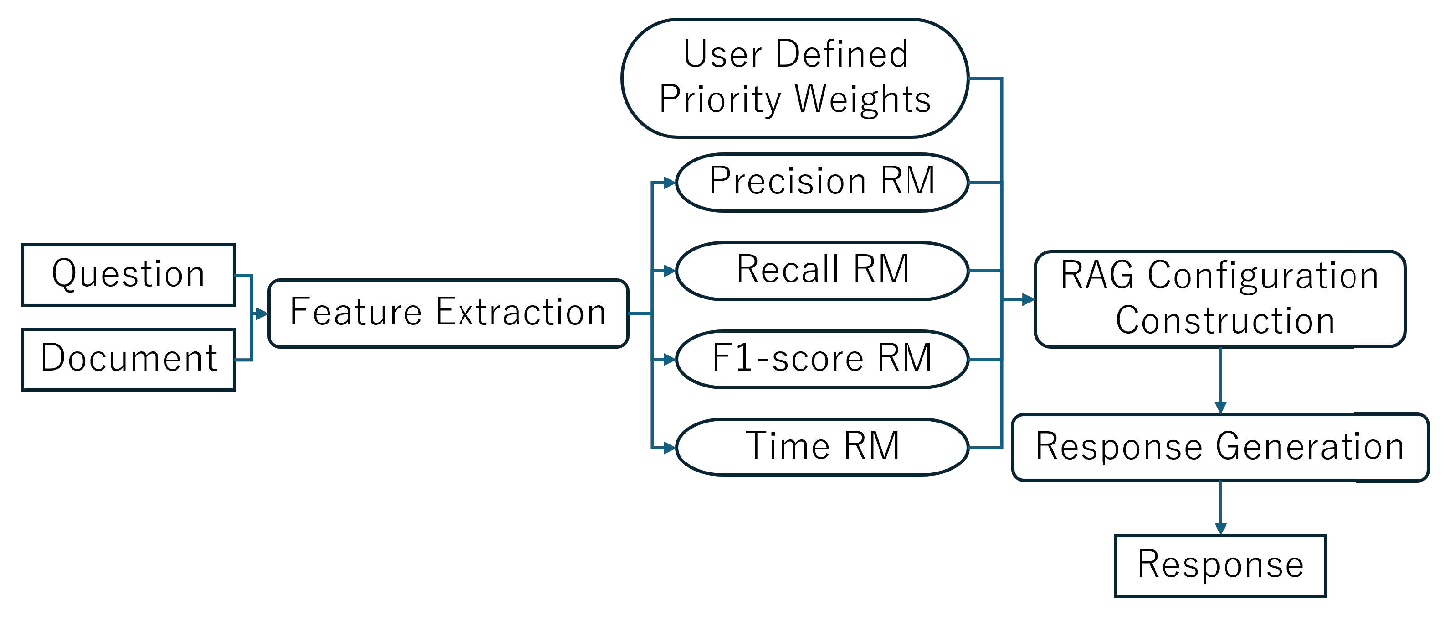
\includegraphics[width=\linewidth]{figures/Fig2}
\caption{Inference procedure of ranking models in the proposed method.}
\label{reasoning}
\end{figure}

In this study, we propose a method that adaptively selects RAG configurations based on query and document features, enabling flexible adjustment of trade-offs between accuracy (precision, recall, $F_1$ score) and cost (execution time). Figures~\ref{construction} and \ref{reasoning} illustrate the training and inference procedures of ranking models (RM) in the proposed method. Precision RM, Recall RM, $F_1$ RM, and Time RM take query/document features and RAG configuration parameters as explanatory variables. These models predict the relative ranks of precision, recall, $F_1$ score, and execution latency, respectively, across candidate RAG configurations. In this section, we describe the proposed method's training and inference components.

\subsection{Feature Extraction} \label{sec3.1}
In this section, we describe how we extract surface-level and semantic features from queries and documents. Assuming one or more candidate documents relevant to the query are available, we extract features during both RM training and inference. These features capture query complexity, user intent, and query-document relevance. We selected 7 features: 4 surface-level and 3 semantic. We selected this set heuristically by evaluating feature combinations and choosing the subset that maximized RM ranking accuracy (detailed ablation analysis is presented in Section~\ref{sec5.5}).

\subsubsection{Surface-level Feature Extraction}
The 4 surface-level features are query token count, query dependency parse tree depth, query type, and document token count.
The query token count reflects not only the query's surface length but also whether it contains multiple conditions, constraints, or modifiers. Generally, longer queries are less likely to contain all required evidence in a single document, increasing the need for multi-document integration.

Query dependency parse tree depth is the maximum reachable path length from the root token during a depth-first traversal of the query's dependency tree. A deeper tree structure indicates nested modifiers and long-range dependencies, requiring greater syntactic integration. From the viewpoint of RAG configuration selection, syntactically complex queries tend to require cross-document evidence synthesis.

Query types are categorized into 4 classes based on expected output: truth-value verification (Yes/No), fact extraction (identifying specific factual information), selection (choosing from the presented options), and passage generation (free-form explanatory description). Classification uses rule-based matching on the query's lowercase leading and specific words. If the leading word is an auxiliary or be-verb (e.g., ``is'', ``can'', ``must''), the query asks whether a statement holds, classifying it as ``truth value verification''. If the leading word is a wh-question word (e.g., ``what'', ``who'', ``where''), it prompts specific fact retrieval and is classified as ``fact extraction''. If the query contains the word ``or'', it is classified as ``selection''. Queries matching none of these rules are assumed to require summary or causal explanation and are classified as ``passage generation''.

The document token count reflects total information volume, as well as potential noise and redundancy. For long documents in particular, chunking adjustments and post-retrieval synthesis strategies significantly affect accuracy and latency, making document length a valuable feature for configuring selection.

\subsubsection{Semantic Feature Extraction}
The 3 semantic features are the cosine similarity between the query and document embeddings, the similarity between keywords extracted from the query and the document, and the cosine similarity between named entities extracted from the query and the document.

Cosine similarity between query and document embeddings measures global semantic alignment. High similarity indicates that a single document likely contains the answer, suggesting that a relatively simple RAG configuration suffices.

Similarity between keywords extracted from query and document evaluates key-point alignment. Because raw documents often contain redundant background text, key evidence in long documents may be buried. Extracting keywords from both query and document and comparing their concatenated representation allows the model to assess key-point consistency.

Cosine similarity between named entities extracted from the query and document compares named entity strings (e.g., persons, organizations, locations, works) present in both texts. Named entities identify core reference targets that strongly influence QA accuracy.

Together, these 3 cosine similarities complementarily capture query-document relevance across full-text, key-point, and entity levels.

\subsection{Dataset Construction} \label{sec3.2}
In this section, we describe the dataset used for RM training, validation, and evaluation. To enable the RM to learn configuration selection rules, we systematically gather performance distributions across a broad configuration space by executing all candidate RAG configurations on training queries and assigning rank labels for relative comparison.

The candidate configuration space comprises 96 combinations across 6 hyperparameter categories shown in Table~\ref{hyperparameters_in_RAG}. We use 3 RAG paradigms: NaiveRAG~\cite{Lewis20}, LightRAG~\cite{Guo25}, and GraphRAG~\cite{edge25}. Retrieval Setting (RS) is set to Stuff or MapReduce for NaiveRAG, and Local or Global for LightRAG and GraphRAG. Chunking settings: Chunk Size (CS) is set to 250 or 500 and Chunk Overlap (CO) to 50 or 100 for NaiveRAG, while CS is 500 or 1000 and CO is 100 or 250 for LightRAG and GraphRAG. Generative Models (GM) are Llama3.1:8b~\cite{Meta24} and Qwen3:14b~\cite{qwen25}, while Embedding Models (EM) are nomic-embed-text~\cite{nussbaum25} and mxbai-embed-large~\footnote{\url{https://www.mixedbread.com/blog/mxbai-embed-large-v1/}}. This comprehensive parameter set ensures sufficient performance variation for RM training.

To build a unified dataset covering 3 heterogeneous RAG paradigms, we standardized configuration parameters as much as possible. We treat the information synthesis strategy (Chain Type) in NaiveRAG as a ``Retrieval Setting'' under the same broad category as LightRAG and GraphRAG retrieval modes. In this paper, we collectively refer to these as ``Retrieval Setting (RS).''

Next, for each execution trial, we record the query ID, configuration parameters, precision, recall, $F_1$ score, and execution latency, and combine these with the extracted features to construct the dataset. Specifically, we evaluate query-document pairs across candidate configurations and compare generated answers against ground-truth references to compute BERTScore-based~\cite{zhang20} precision, recall, and $F_1$ score, along with measured execution latency. BERTScore quantifies semantic similarity between tokens using contextual embeddings without relying on exact string matching, making it ideal for evaluating generated text containing stylistic variations. Relative rank labels (1 to 96) are assigned to precision, recall, $F_1$ score, and execution latency.

\begin{table}[tb]
    \centering
    \footnotesize
    \caption{RAG Configuration Space (96 Total Combinations).}
    \label{hyperparameters_in_RAG}
    \resizebox{\columnwidth}{!}{
    \begin{tabular}{lll}
        \hline
        Parameter & Target RAG & Values \\
        \hline
        \multirow{2}{*}{RAG} & - & \{NaiveRAG, LightRAG, \\ &&GraphRAG\} \\
        \hline
        \multirow{2}{*}{RS} & NaiveRAG & \{Stuff, Map Reduce\} \\ 
        & LightRAG / GraphRAG & \{Local, Global\} \\
        \hline
        \multirow{2}{*}{CS} & NaiveRAG & \{250, 500\} \\ 
        & LightRAG / GraphRAG & \{500, 1000\} \\
        \hline
        \multirow{2}{*}{CO} & NaiveRAG & \{50, 100\} \\ 
        & LightRAG / GraphRAG & \{100 , 250\} \\
        \hline
        \multirow{2}{*}{GM} & \multirow{2}{*}{All RAGs Common} 
        & \{llama3.1:8b, \\ && qwen3:14b\} \\
        \hline
        \multirow{2}{*}{EM} & \multirow{2}{*}{All RAGs Common} 
        & \{nomic-embed-text, \\ && mxbai-embed-large\} \\
        \hline
    \end{tabular}
    }
\end{table}

\subsection{Ranking Model Training} \label{sec3.3}
In this section, we describe the training procedure for RMs that predict configuration rankings using the dataset constructed in Section~\ref{sec3.2}. A key feature of our method is that rather than directly predicting absolute metric values or configurations for a new query, the RM predicts relative rankings among candidate configurations for the same query. This mitigates issues common in regression models—such as score fluctuations caused by query difficulty or measurement noise—enabling robust learning. It also avoids the class imbalance and rank loss inherent in classification approaches, directly optimizing the model to identify top-performing candidate configurations.
The feature vector fed into the RM comprises 13 variables: 7 query/document features and 6 configuration parameters. We train separate RMs for each objective metric (precision, recall, $F_1$ score, and execution time). At inference time, predicted rankings from each objective RM are combined using the aggregated scoring function described in Section~\ref{sec3.4}.

\subsection{RAG Configuration Selection and Top-K Formalization} \label{sec3.4}
Given a new query $q$ and document $d$, the system extracts features and uses trained RMs to predict the rank of each candidate configuration $c \in \mathcal{C}$ ($|\mathcal{C}|=96$) across all evaluation metrics.

\paragraph{Aggregated Scoring Function Background}
To combine multi-objective rankings, we define a composite evaluation score $S(c; q, d)$ for configuration $c$ using a linear combination of reciprocal ranks across objective metrics:
\begin{equation}
\begin{aligned}
S(c; q, d) = & \frac{W_{\mathrm{pre}}}{P_{\mathrm{rank}}(c; q, d)} + \frac{W_{\mathrm{rec}}}{R_{\mathrm{rank}}(c; q, d)} \\
& + \frac{W_{\mathrm{f_1}}}{{F_1}_{\mathrm{rank}}(c; q, d)} + \frac{W_{\mathrm{time}}}{T_{\mathrm{rank}}(c; q, d)}
\end{aligned}
\label{eq1}
\end{equation}
where user-specified priority weights $W$ satisfy:
\begin{equation}
W_{\mathrm{pre}} + W_{\mathrm{rec}} + W_{\mathrm{f_1}} + W_{\mathrm{time}} = 1
\label{eq2}
\end{equation}
Here, $P_{\mathrm{rank}}$, $R_{\mathrm{rank}}$, ${F_1}_{\mathrm{rank}}$, and $T_{\mathrm{rank}}$ denote integer ranks from $1$ to $|\mathcal{C}|$ ($=96$) assigned to configuration $c$ based on predicted values for precision, recall, $F_1$ score, and execution latency, respectively.

The reciprocal rank aggregation scheme offers two primary advantages:
\begin{enumerate}
\item \textbf{Scale Unification and Dominance Prevention}: Combining metrics with vastly different physical scales (e.g., latency in seconds vs. $F_1$ score as a percentage) directly risks having high-magnitude metrics dominate. Converting ranks to reciprocals calibrates all metrics to $(0, 1]$, enabling robust multi-objective optimization.
\item \textbf{High Sensitivity to Top Ranks}: Reciprocal rank $1/r$ produces a large drop between 1st place ($1.0$) and 2nd place ($0.5$), whereas differences between low ranks are negligible, strongly differentiating top-performing candidates.
\end{enumerate}

\paragraph{Top-$K$ Presentation Model Formalization}
In addition to single-configuration presentation ($K=1$), we formalize a practical operational model ($K > 1$) where the top $K$ candidate configurations $\mathcal{C}_K(q, d) \subset \mathcal{C}$ with highest predicted scores are presented to the user.

First, composite scores $S(c; q, d)$ are computed using balanced default weights ($W_{\mathrm{f_1}} = W_{\mathrm{time}} = 0.5$ in Eq.~\eqref{eq1}), and configurations are sorted in descending score order. The subset of top $K$ configurations is defined as $\mathcal{C}_K(q, d)$:
\begin{equation}
\mathcal{C}_K(q, d) = \arg\max^{(K)}_{c \in \mathcal{C}} S_{\mathrm{balanced}}(c; q, d)
\label{eq3}
\end{equation}
where $\arg\max^{(K)}$ extracts the top $K$ scoring elements.

The user executes all configurations within the candidate set $\mathcal{C}_K(q, d)$ and adopts the best-performing configuration $c^*$ ex post according to their operational policy (e.g., accuracy-oriented, precision-oriented, recall-oriented, or time-oriented). For instance, a user adhering to an $F_1$-oriented policy selects:
\begin{equation}
c^* = \arg\max_{c \in \mathcal{C}_K(q, d)} \text{BERTScore}_{F_1}(c)
\label{eq4}
\end{equation}
Under this model, because all candidate configurations in $\mathcal{C}_K(q, d)$ are executed (in parallel or sequentially), total operational latency equals the cumulative execution time of all $K$ configurations. However, user selection compensates for model prediction uncertainty, enabling performance close to oracle upper bounds.

